\chapter{Atmospheric Retrievals}
Everything photon of light that we receive from an exoplanet will interact with its atmosphere, and will therefore provide us with a hint of what that atmosphere may look like.
An atmospheric retrieval is the process of reconstructing the atmosphere of an object based on an observed spectrum.
This process relies heavily on having accurate models which can be parameterized by the physical quantities we are interested in: generally the temperature, pressure and composition \parencite{Madhusudhan2018}.
As these models cover a very large parameter space (>10 parameters, each covering several orders of magnitude), it is necessary to have an efficient method for sampling this space, computing a model and comparing this model to the data 
\parencite{Benneke2012,Benneke2013}.
Currently, atmospheric retrieval methods have been used for both exoplanets and brown dwarfs to identify water, methane, CO, CO$_{2}$ and other species \parencite{Konopacky2013,Barman2015}, along with clouds being a universal feature \parencite{Line2017,Schlawin2018,Morley2018}

This chapter will outline the process of an atmospheric retrieval from modeling to marginalization of posteriors, and will examine the impact that the instrumental effects described in Chapter \ref{ch:fringe} have on the retrieved parameters. 
Additionally, this will provide an example of how the MIRI MRS can be used to explore exoplanet and brown dwarf atmospheres, and what observational parameters should be considered when studying these objects, following similar studies from \parencite{Batalha2018,Schlawin2018} for NIRSpec and LRS observations and \parencite{Feng2018} for future reflected light missions.


 %atmo ret,basically everything nested samp, 
%\cite{Fisher2019} %Cross corr machine learning hoeijmakers
%\cite{Oreshenko2019}% Model grid comparison random forest
%\cite{Barman2015} %HR8799b water methan CO 

%\cite{Blanco-Cuaresma2018} %Stel spec caveats
%\cite{Konopacky2013} %CO and water in hr8799

%\parencite{Morley2018} %D/H ratios
%\cite{Lupu2016} %Is actually 2016 - reflected light atmo rets (multinest)
%\cite{Gandhi2018} %HyDRA retrieval code
%\cite{Baudino2017} %Troublesome model params
%\cite{Line2013} %Secondary eclipse retrieval technique comparison
%\cite{Madhusudhan2018b} % With Seagar - temp nad abundance retrieval pt profile
%\cite{Irwin2008} %Nemisis atmo ret code
%\cite{Robinson2016} %Observations of planets with coronographs in space %(WFIRST)
%\cite{Waldmann2015} %TauRex
%\cite{Waldmann2015a} %TauRex emission
%\cite{Line2015,Line2017,Zalesky2019} % Brown dwarf retrieval part 1,2,3

%\cite{Batalha2018}%MIRI LRS - strategies (obs)
% Gravity Beta Pic - petitRadTrans retrieval how to, CO
%\cite{Feng2018} %Future ref light: basis of mine but emission
%\cite{Molliere2019}% Two papers, isotopologues and petitRadTrans
\subsubsection{Atmospheric Modeling}
Atmospheric modeling is the task of creating an spectra based on the physical properties of the atmosphere.
This is a broad task that can range from a 3D Global Circulation Model (GCM) which accounts for self-consistent atmospheric chemistry \parencite{Chen2019} to a 1D model based around an empirical temperature-pressure profile \parencite{Molliere2019}.
The choice of model depends largely on the requirements for accuracy and computational cost. 
Considering the potentially millions of possible atmospheres that must be examined in a retrieval problem, whatever model is used must be computationally efficient while still maintaining a close approximation of reality.

%\cite{Zhang2019} %PLATON Transmission spectra generation
\section{petitRADTRANS}
For this work we chose to use the petitRADTRANS package due to its user-friendly python implementation, high speed computation for retrieval use and extensive high resolution, line-by-line spectral library for generating planetary spectra \parencite{Molliere2019}. 
It is a 1D, radiative transfer package with many parameters options, described in table \ref{tab:petitradparams}
PetitRADTRANS can compute both emission and transmission spectra, with an output spectral resolution of R=1000 in correlated k mode, or R=1 000 000 in line-by-line mode. 

\begin{table}[t]
	\centering
	\begin{tabular}{ll}
		\toprule
		\textbf{Property} & \textbf{Description}\\
		\midrule
		Temperature & Parameterized, e.g. \parencite{Guillot2010}\\
		Abundances & Parameterized, e.g. vertically constant\\
		Scattering & Cloud scattering, transmission spectra only\\
		Clouds & Power law and condensation clouds\\
		Cloud particle size & $f_{SED}$ and K$_{ZZ}$ or parameterized\\
		Particle size distribution & log-normal, variable width\\
		Cloud abundance & Parameterized\\
		Wavelength spacing & R=1000 (c-k), 10$^{6}$ (lbl)\\
		Valid emission spectra & Clear, from NIR and longer\\
		\bottomrule
	\end{tabular}
	\caption{Description of the parameters available in petitRADTRANS. For cloud particles, $f_{SED}$ is the mass-averaged ratio of the cloud particle settling speed and mixing velocity. K$_{ZZ}$ is the atmospheric eddy diffusion coefficient \parencite{Ackerman2001}}
	\label{tab:petitradparams}
\end{table}

Note that much of the following sections applies to many other similar 1D radiative transfer atmospheric modelling programs such as ATMO \parencite{Goyal2019}, Planetary Spectrum Generator \parencite{Villanueva2018}, HELIOS \parencite{Malik2017,Malik2019} and others.
Many (or even most) of these programs rely on the same set of high-resolution molecular line lists, including HITRAN/HITEMP \parencite{Rothman1981,Rothman2010,Gordon2017}, ExoMol/ExoCross \parencite{Tennyson2016,Tennyson2017,Yurchenko2018} and others. 
%\cite{Behmard2019}%Cool star spectroscopy, hires

\subsection{Radiative Transfer}
In order to compute the emission spectrum an initial featureless blackbody spectrum $B(T_{int})$ is passed through multiple discrete layers of the atmosphere, parameterized by their temperature, pressure, and the opacities of each of the species present in a given layer.
Modeling each layer as plane parallel, the intensity is computed as in \parencite{Irwin2008,Molliere2017,Molliere2019}
\begin{equation}
I_{top} = B(T_{int})\mathcal{T}^{atmo} + \frac{1}{2}\sum_{i=0}^{N_{L}-1}\left[B(T^{i}) + B(T^{i+1})\right]\left(\mathcal{T}^{i}-\mathcal{T}^{i+1}\right)
\end{equation}
$N_{L}$ is the number of layers in the atmosphere, and $\mathcal{T}$ is the transmission from a given layer to the top of the atmosphere. All quantities are averaged per wavelength bin in c-k mode, while they are evaluated at each wavelength point in line-by-line mode.

In order to compute the temperature structure of the atmosphere, a modified Guillot model \parencite{Guillot2010} was used, as used in \parencite{Molliere2017,Molliere2019}.
The temperature structure is defined as 
\begin{equation}
T(P) = \left<T_{Guillot}(P)\left(1-\frac{\alpha}{1+P/P_{trans}}\right)\right>_{P}.
\end{equation}
As denoted by $\left<\right>_{P}$, this profile is boxcar-smoothed over log(P), with bin widths of 1.25 dex \parencite{Molliere2019}. 
The modified Guillot profile is defined as
\begin{align}
T_{Guillot}(P) &= \frac{3T^{4}_{int}}{4}\left(\frac{2}{3} + \delta P\right)\\
&+\frac{3T^{4}_{eq}}{4}\left[\frac{2}{3} + \frac{1}{\gamma\sqrt{3}} + \left(\frac{\gamma}{\sqrt{3}} - \frac{1}{\gamma\sqrt{3}}\right)e^{-\gamma\delta\sqrt{3}P}\right]
\end{align}
with the second term accounting for irradiation of the upper atmosphere.
The opacity parameters $\delta=\kappa_{IR}/g$ and  $\gamma=\kappa_{V}/\kappa_{IR}$ are defined such that the optical depth $\tau=\delta\cdot P$. 
$T_{int}$ is the internal temperature of the planet, and is equivalent to the effective temperature of the planet, that is the temperature of a blackbody with the same luminosity as itself.
$T_{eq}$ is the equilibrium temperature of the planet, based on the temperature of the host star and separation of the planet. 
For an isolated, free floating object this temperature goes to 0.
The remaining free parameters $\alpha$, $P_{trans}$ simply modify the shape of the temperature structure according to the pressure.

\subsection{Opacity Sources}
To compute the emission spectra of an atmosphere, petitRADTRANS accounts for various opacity contributions including absorption and emission lines, collisionally induced absorption, cloud opacity and scattering and Rayleigh scattering cross sections. These sources are described in detail in \parencite{Molliere2019}, summarized in tables 2 and 3. For this work we consider only the case of a cloud-free atmosphere due to the complexity of realistic cloud modeling.
\subsubsection{Line-by-line}
In its high resolution line-by-line mode, petitRADTRANS computes emission spectra with R=10$^{6}$. 
These spectra are computed using opacity sources for molecular and atomic lines from ExoMol/ExoCross library \parencite{Yurchenko2018}. Pressure broadening is taken into account using the coefficients from HITRAN/HITEMP \parencite{Rothman2010,Rothman2013} or from \parencite{Sharp2007} (Eqn. 15). The line opacities are computed from 80-3000K, and from 0.3-28$\mu$m in high resolution mode.
\subsubsection{Correlated K}
The low resolution mode of petitRADTRANS uses the correlated-k (c-k) method of computing line opacities \parencite{Goody1989,Lacis1991,Fu1992}. 
This method for calculating emission and absorption features assumes that the opacity distribution functions between differing species are uncorrelated, which permits simple computation of overlapping features. 
While petitRADTRANS implements a c-k method with a spectral resolution of 1000, in principle it is accurate to much higher resolutions.
However, the principle utility of the c-k method is in the dramatic reduction in computational cost for computing a spectra such that petitRADTRANS can be used as the foundation for an atmospheric retrieval code requiring hundreds of thousands or millions of models to be generated. 
\parencite{Molliere2019} discusses the variations between the results of the line-by-line method and the c-k method, finding discrepancy of at most 6\%.
Typical variation is much lower, as seen in Fig. 2 of \parencite{Molliere2019}.

\subsubsection{Clouds}
While clouds are a seemingly universal feature in exoplanets and brown dwarfs \parencite{Morley2014,Line2016,Faherty2018}, they remain a difficult problem for retrieval studies. 
Clouds form when a species condenses out of the gas phase, typically around a small nucleus.
This creates a layer of particles at a reasonably well defined altitude in the atmosphere, and prevents the observation of deeper atmospheric layers.
While a simple model of clouds may be a `gray' cloud deck that acts uniformly across wavelength, a more complex model will account for differing IR and visible opacities, as well as particle scattering and other complex microphysics.
From experience on Earth and within the solar system, cloud systems are highly complex and variable, with shifting cloud coverage and structure.
The mid infrared in particular may allow for an observational window to probe deeper atmospheric layers and begin to characterize cloud composition.
In current retrieval codes, clouds are generally designed from a simple model based on a given particle distribution \parencite{Ackerman2001}, or simply as a gray cloud deck at a specified pressure level.
Both of these models are implemented in petitRADTRANS.
These models do not agree well with microphysical models, and lead to substantial difficulties in the interpretation of retrieved spectra.
This remains an open problem for atmospheric retrievals, and we do not attempt to examine cloud effects in this work, instead choosing the simple, though unrealistic case of a clear atmosphere. 
\parencite{Schlawin2018} examines potential impacts of clouds on atmospheric retrievals with the MIRI LRS.

\section{Bayesian Inference}
An atmospheric retrieval is the process of extracting information about physical parameters from a measured spectrum. 
In general this procedure involves comparing the data to a series of template spectra with known parameters and identifying the best fit model.
Unfortunately for astronomers, atmospheres are complicated: typical one 1D models still require many (>15) parameters to generate a somewhat realistic model. 
This results in a very large parameter space in which to search for the correct set of properties that describe our measurement.

Monte Carlo methods, including Nested Sampling, are used to effectively search this large space using the Baysian evidence as a goodness-of-fit metric.
Here we will follow \parencite{Speagle2019} to provide a brief overview of Bayesian inference.

To measure the likelihood of a given model, we turn to Bayes' Theorem:
\begin{equation}\label{eqn:bayes}
P(\mathbf{\Theta}_{M}|\mathbf{D},M) = \frac{P(\mathbf{D}|\mathbf{\Theta},M)P(\mathbf{\Theta}|M)}{P(\mathbf{D}|M)}
\end{equation}
In our notation, $\mathbf{\Theta}$ is the set of parameters that describe a model $M$, that is fit to the data $\mathbf{D}$. 
Bayes' theorem asks what is the probability that the parameters $\mathbf{\Theta}$ are true given the data and model. 
The distributions for each parameter are the \textbf{posterior} distributions.

This is then related to the \textbf{likelihood} $P(\mathbf{D}|\mathbf{\Theta},M)$ of measuring the data given the model, the \textbf{prior} probability $P(\mathbf{\Theta}|M)$ which describes our degree of belief in our model and the \textbf{evidence} $P(\mathbf{D}|M)$, which is marginalized over all possible $\mathbf{\Theta}$ and quantifies how well the model describes the data.
To simplify notation, we adopt the following convention for Bayes' theorem:
\begin{equation}
\mathcal{P}(\mathbf{\Theta}) = \frac{\mathcal{L}(\mathbf{\Theta})\pi(\mathbf{\Theta})}{\mathcal{Z}}
\end{equation}

In general, the goal of an atmospheric retrieval is to find the best fit model by maximizing the evidence $\mathcal{Z}$, and as a by product finding the marginalized posterior distributions for each parameter.
This comes with many challenges, especially when dealing with large numbers of parameters.
Selection of the priors and model will determine the extent to which a result can be interpreted, while sampling large parameter spaces and computing likelihoods introduces substantial numerical challenges. 
The Markov Chain Monte Carlo method and the Nested Sampling method described below attempt to solve the challenges of exploring a large parameter space.
\subsection{MCMC}
\cite{Foreman-Mackey2013} %emcee
\cite{MacKay2003} %MCMC
\subsection{Nested Sampling}
Nested sampling attempts to address several of the shortcomings of MCMC methods while simultaneously improving computational efficiency \parencite{Skilling2004}.
A particular strength of the method is in the sampling of highly multimodal distributions, removing the problem where an MCMC approach may get stuck in a single local maximum.
MCMC methods generate samples `proportional to' the true posterior distributions, which lead to difficulties in computing the evidence $\mathcal{Z}$ \parencite{Speagle2020}. 
In contrast, nested sampling puts the evidence first and provides estimates of the posterior distributions from the importance weights of the final set of samples. First described in \parencite{Skilling2004}, nested sampling has been adopted as the sampling algorithm of choice within the astrophysics community \parencite{Feroz2009,Buchner2014,Feroz2019,Speagle2020}.

With the goal of parameter estimation, nested sampling attempts to estimate the evidence $\mathcal{Z}$ rather than directly sampling the posteriors \parencite{Skilling2004}. 
This is done by integrating over the entire parameter space of $\mathbf{\Theta}$
\begin{equation}
\mathcal{Z} = \int_{\Omega_{\mathbf{\Theta}}}\mathcal{L}(\mathbf{\Theta})\pi(\mathbf{\Theta})d\mathbf{\Theta}
\end{equation}
This is difficult.

Rather than attempting to directly solve the entire multidimensional integral, nested sampling transforms this into an integration over the \textit{prior} volume X:
\begin{equation}
\mathcal{Z} = \int_{\Omega_{\mathbf{\Theta}}}\mathcal{L}(\mathbf{\Theta})\pi(\mathbf{\Theta})d\mathbf{\Theta} = \int_{0}^{1}\mathcal{L}(X)dX
\end{equation}
This is now a contour integral over isocontours $\mathcal{L}(X)$ which bound the prior volume
\begin{equation}
X(\lambda) = \int_{\Omega_{\mathbf{\Theta}}:\mathcal{L}(\mathbf{\Theta})\geq\lambda}\pi(\mathbf{\Theta})d\mathbf{\Theta}
\end{equation} 
which is the fraction of the prior where the likelihood of the data given the model is above some threshold $\lambda$.
The integration is now simplified into a 1D integration over X, given proper prior selection.

\subsubsection{Method}
Consider a parameter space with $D$ dimensions.
We will describe this space as a unit hypercube, where each parameter runs from 0 to 1.
Priors are thus transformations from this space to a physical parameter space.
Often the prior is a uniform distribution, which simply scales the space, but it may also be an informative prior such as a normal distribution centered at an expected physical value.
In order to sample this space, $N_{L}$ `live points' are generated, each of which provides a set of parameters $\mathbf{\Theta}$. 
$N_{L}$ must be greater than $D+1$, and typically values on the order of $50\times D$ are used \parencite{Feroz2009}.
Using a likelihood function $\mathcal{L}(\mathbf{\Theta})$, the evidence $\mathcal{Z}$ can be computed by comparing the model to the data.
Having computed the evidence at each point, the live points are then sorted and the point with the lowest evidence is discarded.
A set of ellipsoids is drawn around the remaining points. 
The procedure for computing these ellipsoids is given in \parencite{Feroz2008,Feroz2009}.
By using a set of ellipsoids, multiple modes in the parameter space can be encompassed.
Once the ellipsoids bounding the remaining points are drawn, a new sample is drawn from within the restricted sample space.
The evidence for the new point is computed, and it is accepted if the evidence is greater than the minimum evidence of the previous remaining set of points.
The entire procedure is repeated until some convergence criteria is satisfied, with each iteration resulting in a smaller volume being encompassed by the ellipsoids, nested within the previous volume.

This procedure can be improved in many ways, including importance nested sampling \parencite{Feroz2019} and dyamic nested sampling \parencite{Speagle2020}. 

\subsection{Multinest}
For our implementation of an atmospheric retrieval code, we chose to use the Multinest algorithm \parencite{Feroz2009} using the pyMultinest wrapper \parencite{Buchner2014} and using importance nested sampling to improve the accuracy of the Bayesian evidence calculation \parencite{Feroz2019}.
This particular implementation of nested sampling is commonly used in atmospheric retrieval codes due to its fast Fortran implementation, though it was initially developed for cosmological problems.

Using the pyMultinest package, we implemented the required log-prior function which transforms the unit hypercube to physical parameter space and the log-likelihood function used to compare the model to the data. The full code is available at \url{https://github.com/nenasedk/petitRetrieval}, and is based of the emission spectrum retrieval described in \parencite{Molliere2019}. 
Retrievals were typically performed using 500 or 1000 live points, with the convergence criteria 
\begin{equation}
\Delta\ln\mathcal{Z} = \ln{Z_{i} - Z_{i+1}}
\end{equation}
set to 0.3 for parameter estimation and 0.8 for model comparison, as suggested in the pyMultinest documentation.

\section{Observations}\label{sec:obs}
The targets used in our retrieval study are guided by the JWST ERS and GTO programs. This allows us to use well-defined observing strategies for each object, and present a clear case for the science that can be accomplished with these observations.
While all three were discussed in Chapter 1, we will now outline the proposed observing strategies and science cases for each target.
\subsubsection{VHS-1256B}
VHS-1256b is a young (0.2Gyr), high mass (11.2M$_{Jup}$) planet at a distance of 12.7pc \parencite{Bowler2016}. 
The wide separation of 8" makes it an easy target for observation with the MRS, as its host star will fall outside of the FoV.
It has a J-band magnitude of 16.662, and a late L spectral type \parencite{Miles2018}.
As an object of interest for the JWST ERS program 1386, it will be observed with the NIRCam imager, along with both the NIRSpec and MRS spectrometers \parencite{Hinkley2019}.
Using the MRS, VHS-1256b will be observed using a SLOW readout pattern, using 30 groups per integration, with one integration per exposure using a 2 point dither pattern.
This results in a total exposure time of 1433.395s in each of the MRS sub-bands, and will cover the full wavelength range of the MRS.
It will be simultaneously imaged using the MIRIM instrument.
An additional background only exposure will be taken using the same exposure parameters, but without dithering, for a total of half of the science exposure time.

Methane spectral features have been detected in the L-band spectrum of VHS-1256b \parencite{Miles2018}, but mid infrared spectroscopy will allow the use of methane and other molecules to characterize atmospheric properties such as dis-equilibrium chemistry and vertical mixing \parencite{Beichman2019}. 
\subsubsection{2M1207b}
2M1207b is a 1600K, 10 M$_{Jup}$ object at wide separation from its brown dwarf primary (TWA 27) and a distance of 52.4pc \parencite{Bowler2016}.
In comparison to VHS-1256b, 2M1207b has a relatively small separation of 0.77", which is more characteristic of currently known objects.
As one of the first directly imaged exoplanets, it provides a template for characterizing young, hot objects, and will be observed in the JWST GTO program 1270 \parencite{Birkmann2019}.
This observation will use the NIRSpec IFU, MIRIM and the MIRI MRS.

Using the MRS, 2M1207b will be observed using a FAST readout to prevent detector saturation, using 76 groups per integration, and one integration per exposure. 
It will use a 4 exposure dither pattern, for a total integration time of 843.612s per sub-band, covering the full wavelength range of the MRS. 
Combined with the NIRSpec observation, this will provide a continuous spectrum over the entire JWST wavelength range.
The host star of 2M1207b is faint, allowing for good enough contrast for a straightforward observation \parencite{Beichman2019}.
\subsubsection{WISE 0855-0714}
Although it is a Y-type brown dwarf, WISE 0855 is the most similar known object to Jupiter outside our solar system that has been directly observed \parencite{Luhman2014}. 
At 250K, WISE 0855 is very faint, with an H-band magnitude of 25, but its proximity at 2pc makes it an ideal target for characterization.
The JWST GTO Program 1230 will observe WISE 0855 using NIRCam, NIRSpec and the MIRI MRS \parencite{Oliveira2019}.
It will use a FAST readout, with 180 groups per integration, and one integration per exposure for a total of 999s of integration time for each sub-band. No dithering will be used.

As a cold object, WISE 0855 provides the best known extra-solar template for older planetary mass objects.
With the improved sensitivity and long wavelength coverage of JWST, it is hoped that more low mass and colder exoplanets may be directly imaged.
Understanding the atmosphere of WISE 0855 will provide a great deal of insight for the challenges of such exoplanetary atmospheres. 
Clouds are suspected to be present \parencite{Faherty2018}, a feature which will be better understood using mid infrared observations.

\begin{table}[t]
	\centering
	\begin{tabular}{l|ccc}
		\toprule
		\textbf{Parameter} & \textbf{VHS-1256b} & \textbf{2M1207b} & \textbf{WISE 0855}\\
		\midrule
		ObsDate & 0.0 & 0.0 & 0.0\\
		Path & SHORT/LONG & SHORT/LONG & SHORT/LONG\\
		Dither & 2 point & 4-point & None\\
		Disperser & ALL & ALL & ALL\\
		Detector & SW/LW & SW/LW & SW/LW\\
		MRS Mode & SLOW & SLOW & FAST\\
		Exposures & 1 & 1 & 1\\
		Integrations & 1 & 1 & 1\\
		Groups & 30 & 76 & 180\\
		Cosmic Rays & None & None & None\\
		\bottomrule
	\end{tabular}
	\caption[Observation Parameters]{Observing parameters for each selected target. Observation parameters are based on JWST proposals, and set in order to cover channels 1 through 3. For the disperser, ALL implies running a simulation for each of the SHORT/MEDIUM/LONG sub-bands. A total of 6 simulations are necessary to cover the entire wavelength range. Cosmic rays are turned off due to issues with MIRISIM.}
	\label{tab:obsparams}
\end{table}
\subsubsection{Science Goals}
Atmospheric retrievals are currently the best tools for characterizing the composition and structure of exoplanet atmospheres. 
Parameters such as the C/O ratio may trace the formation history of planets, and may be able to settle the debate between gravitational instability and core accretion formation models \parencite{Madhusudhan2012,Moses2013}.
From solar system observations, along with our own experience on Earth, we know atmospheres are constantly changing, and time series observations will open the door to investigation of dynamics and variability.
Understanding the composition and chemistry of these atmospheres will also provide insight into the diversity - and similarity - between these systems.
Clouds are poorly understood within our own solar system, and are certain to be present in the atmospheres of other worlds.
Perhaps the most interesting prospect is uncovering novel features that have not yet been predicted, and will open the door to new avenues of exploration.

For this work, we are primarily concerned with constraining the ability of the MRS to retrieve known input parameters. 
With simulated spectra from petitRADTRANS providing a ground truth, we can compare the results of retrievals over a range of fringing cases.
%\subsection{Atmospheric Parameters}
%% CO ratio for characterization
%\cite{Garland2019} %BD absorption
%\cite{Fegley1994} %Jupiter/Saturn atmospheres
%\cite{Tokunaga1983} %MIR atmosphere spectra
\section{Methods}
Here we will outline how we generated our input spectra, and the procedure we used to perform our atmospheric retrieval.
\subsection{Spectra Generation}
\begin{figure}[t]
	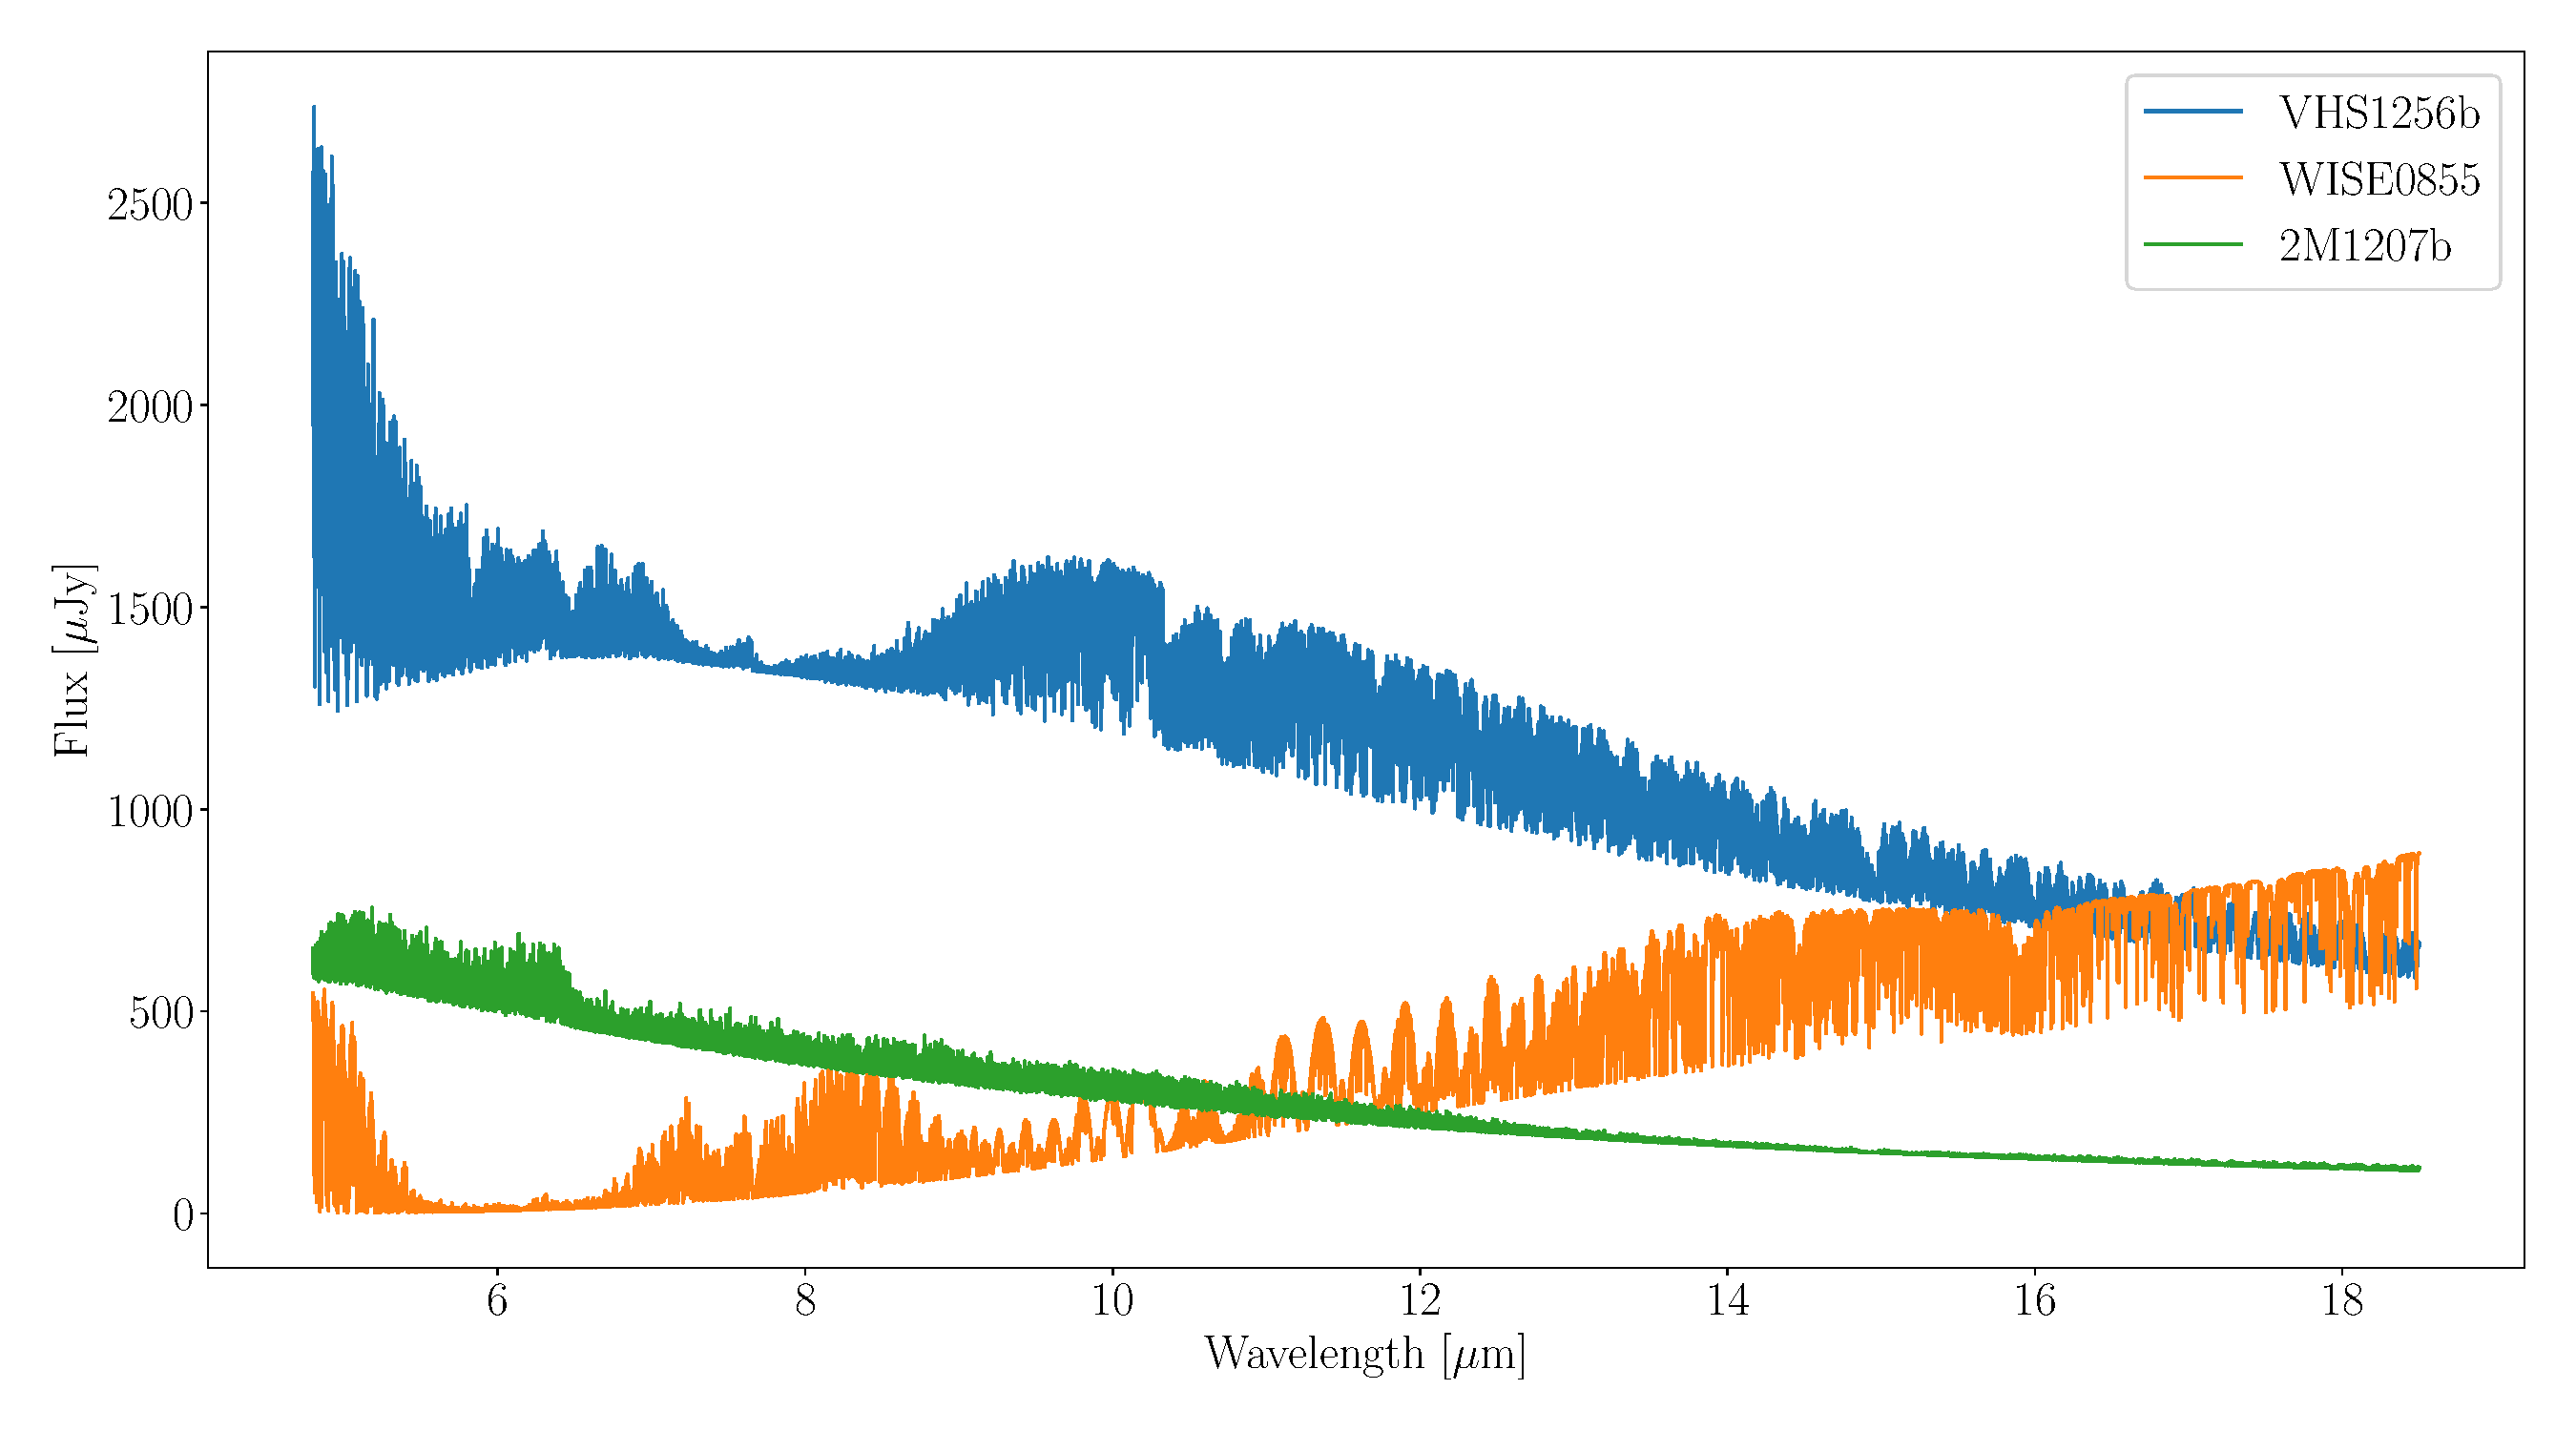
\includegraphics[width=\linewidth]{petitInputSpectra}
	\caption{High resolution spectra generated by petitRADTRANS for each of the simulated targets.}
	\label{fig:petitinput}
\end{figure}
We used petitRADTRANS in high resolution, line-by-line mode in order to calculate a spectrum that can be passed as input to MIRISIM.
All three input spectra used are shown in Fig. \ref{fig:petitinput}.
The parameters chosen for each target are given in table \ref{tab:inputparams}. 
All spectra cover a range of 4.8-18.5 micron in order to fully cover channels 1 through 3 of the MRS. 
Channel 4 is ignored due to photometric calibration issues and lack of sensitivity to faint sources.

The spectra generated by petitRADTRANS are in terms of the emitted flux and are in units of erg cm$^{-2}$ m$^{-2}$ s$^{-1}$ $Hz^{-1}$. 
MIRISIM requires the flux incident on the detector in units of $\mu$Jy, so we convert the as 
\begin{equation}
F_{inc} [\mu\textrm{Jy}] = 10^{29}\times F_{em} \times \left(\frac{R_{pl}}{d_{pl}}\right)^{2}
\end{equation}
The wavelength grid produced by petitRADTRANS is log-spaced, and we use the \verb|spectres| python package \parencite{Carnall2017} in order to convert to a linear spaced grid with R=12000 at 4.0$\mu$m. 
This ensures the input spectrum will oversample the instrumental spectral resolution by a factor of at least 4 across the whole wavelength range.

While it is possible to add a background term to a spectrum using MIRISIM, we chose not to use any background in order to improve our spectral extraction after processing with the JWST pipeline, with the understanding that errors from background subtraction will be negligible in actual data.
\begin{table}[t]
	\centering
	\begin{tabular}{l|ccc}
		\toprule
		\textbf{Parameter} & \textbf{VHS-1256b} & \textbf{2M1207b} & \textbf{WISE 0855}\\
		\midrule
		Radius [R$_Jup$] & 1.29 & 1.5 & 1.17\\
		Distance [pc] & 12.7 & 52.4 & 2.23\\
		$\log g$ & 4.25 & 3.2 & 4\\
		$T_{int}$ [K]& 900 & 1600 & 250\\
		$T_{equ}$ [K]& 3.4 & 10 & 3.4\\
		$\kappa_{IR}$ & 0.01 & 0.01 & 0.01\\
		$\gamma$ & 0.3 & 0.4 & 0.3\\
		\midrule
		\multicolumn{4}{c}{\textbf{Abundances}}\\
		\midrule
		 H$_{2}$ & 0.898 & 0.74 & 0.73\\
		 He & 0.102 & 0.24 & 0.25\\
		 H$_{2}$O & 1$\times10^{-3}$ & 5$\times10^{-3}$ & 5$\times10^{-4}$\\
		 CO & 1$\times10^{-7}$& 1$\times10^{-2}$ & 1$\times10^{-15}$\\
		 CO$_{2}$ & 1$\times10^{-5}$& 1$\times10^{-3}$ & 1$\times10^{-14}$\\
		 CH$_{4}$ & 3$\times10^{-3}$& 1$\times10^{-6}$ & 3$\times10^{-4}$\\
		 NH$_{3}$ & 1$\times10^{-5}$& 1$\times10^{-7}$ & 3$\times10^{-3}$\\
		 C$_{2}$H$_{2}$ & 1$\times10^{-8}$& 1$\times10^{-9}$& \ldots \\
		 HCN & 1$\times10^{-10}$ & 1$\times10^{-9}$ & 1$\times10^{-9}$ \\
		 TiO & \ldots & 5$\times10^{-7}$ & \ldots \\
		 SiO & 1$\times10^{-6}$ &  \ldots & \ldots \\
		\bottomrule
	\end{tabular}
	\caption[petitRADTRANS inputs.]{Input parameters to generate spectra using petitRADTRANS. High resolution line-by-line mode was used. $\kappa_{IR}$ and $\gamma$ are the infrared opacity and ratio of visible to IR opacities respectively. The values chosen for these parameters are based on \parencite{Molliere2019}. The abundances chosen are arbitrary values chosen to encompass a wide range of compositions and to test the ability of the retrieval code to recover small abundances. Where possible, values were chosen to qualitatively reflect known species present \parencite{Miles2018}. }
	\label{tab:inputparams}
\end{table}
\subsection{Atmospheric Retrieval Setup}
\subsubsection{Prior choice}
The choice of priors is a consistent challenge when using a Bayesian framework.
When performing a free-retrieval, uninformative priors must be chosen to allow the data to drive the posterior distribution.
This can lead to unphysical solutions or combinations of parameters.
The alternative is to use physically motivated priors, at the risk of missing unexpected phenomena.

We based our prior selection on the choices made in \parencite{Molliere2019}.
We use an uninformative uniform distribution on the temperature parameters, as well as on the log of abundance, gravity and pressure parameters.
Uniformly drawing from the log of the parameters allows for better coverage of the very large parameter space (from 10$^{-15}$ to $10^{0}$ in each of the fractional abundances).
For the opacity parameters $\gamma,\delta$ and $\alpha$ we use a normal distribution centered around the expected value. 

Trial runs showed that the posterior distributions for these parameters are not driven by the priors.
Our prior choices and the ranges over which they cover are given in table \ref{tab:priors}.
% Uniform in log space
% Gaussian/normal for some
% based on petitRadTrans paper
\begin{table}[t]
	\centering
	\begin{tabular}{lll}
		\toprule
		\textbf{Parameter} & \textbf{Prior} & \textbf{Constraints}\\
		\midrule
		$\log\delta$ & $\mathcal{N}(-5.5,2.5)$&\\
		$\log\gamma$ & $\mathcal{N}(0,2)$&\\
		T$_{int}$ & $\mathcal{U}(0,3500)$&\\
		T$_{equ}$ & $\mathcal{U}(0,30)$&\\
		$\log P_{Trans}$ & $\mathcal{N}(-3,3)$&\\
		$\alpha$ & $\mathcal{N}(0.25,0.4)$&$\alpha < 1$\\
		$\log g$ & $\mathcal{U}(2.0,4.5)$&\\
		$\log P_{0}$ & $\mathcal{U}(-5,2)$&\\
		$\ln(X_{i})$ & $\mathcal{U}(-18,0)$ & $\sum X_{i} < 1$\\
		\bottomrule		
	\end{tabular}
	\caption{Prior choices for atmospheric retrievals. $\mathcal{U}(a,b)$ is a uniform distribution from $a$ to $b$. $\mathcal{N}(\mu,\sigma)$ is a normal distribution. $T_{int}$ corresponds to the effective temperature of an object, while $T_{equ}$ is the equilibrium temperature between an object and a host star. For free floating objects, $T_{equ}$ is set to 3.4K, justifying the small range of the prior. $\delta$ is in units of bar$^{-1}$, temperatures are in K, and pressures in bar.}
	\label{tab:priors}
\end{table}

\section{Results}
\subsection{Model Selection}
\begin{figure}[h]
	%\includegraphics[content...]{imagefile}
	\caption{Bayesian evidence for models of differing dimensionality.}
	\label{fig:bicdim}
\end{figure}
% Number of parameters
% Bayesian evidence
\subsection{Fringing Comparison}
PRELIMINARY PLOTS NOT FINAL
\begin{figure}[h]
	%\includegraphics[content...]{imagefile}
	\caption{Posterior Distributions for XX for different fringe cases}
	\label{fig:postfringe}
\end{figure}
% Bias of different parameters
% Different widths
% Detection of non-existant species
\subsection{VHS-1256b}
\begin{figure}[h]
	%\includegraphics[content...]{imagefile}
	\caption{Posterior Distributions for}
	\label{fig:postVHS}
\end{figure}
\begin{figure}[h]
	%\includegraphics[content...]{imagefile}
	\caption{Pressure Temperature profile for}
	\label{fig:presVHS}
\end{figure}
\begin{figure}[h]
	%\includegraphics[content...]{imagefile}
	\caption{Best fit model for}
	\label{fig:bestfitVHS}
\end{figure}

\subsection{2M1207b}
\begin{figure}[h]
	\includegraphics[width=\linewidth]{2M1207B_v2_fringing_corner}
	\caption{Posterior Distributions for 2M1207b.}
	\label{fig:post2M}
\end{figure}
\begin{figure}[h]
	%\includegraphics[content...]{imagefile}
	\caption{Pressure Temperature profile for}
	\label{fig:pres2M}
\end{figure}
\begin{figure}[h]
	%\includegraphics[content...]{imagefile}
	\caption{Best fit model for}
	\label{fig:bestfit2M}
\end{figure}

\subsection{WISE 0855}
\begin{figure}[h]
	%\includegraphics[content...]{imagefile}
	\caption{Posterior Distributions for}
	\label{fig:postWISE}
\end{figure}
\begin{figure}[h]
	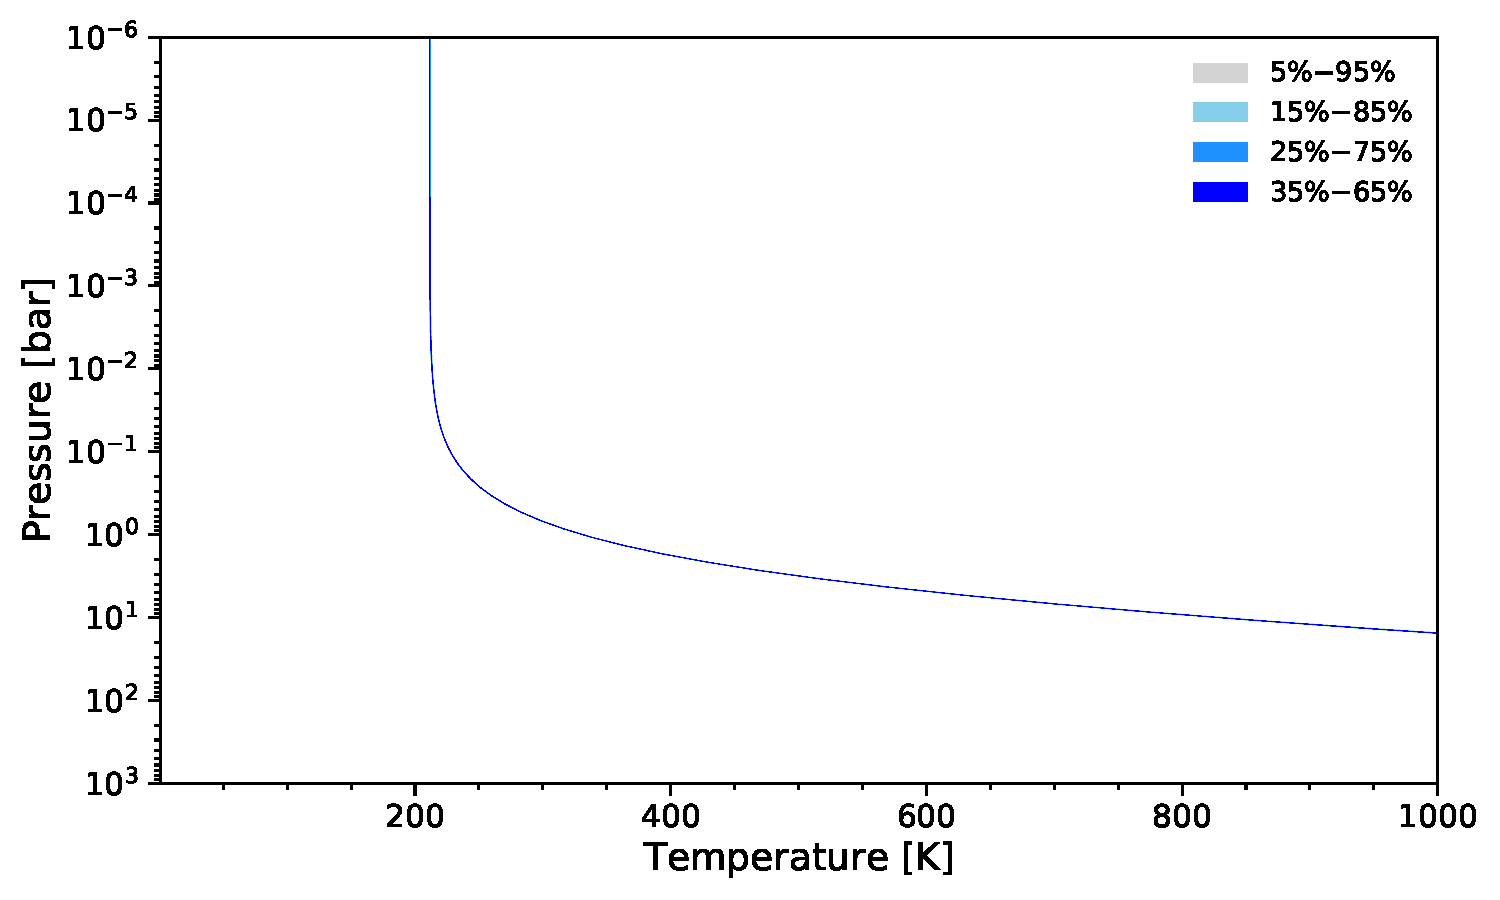
\includegraphics[width=\linewidth]{WISE0855_ptsrc_onax_pt_env}
	\caption{Pressure Temperature profile for WISE 0855.}
	\label{fig:presWISE}
\end{figure}
\begin{figure}[h]
	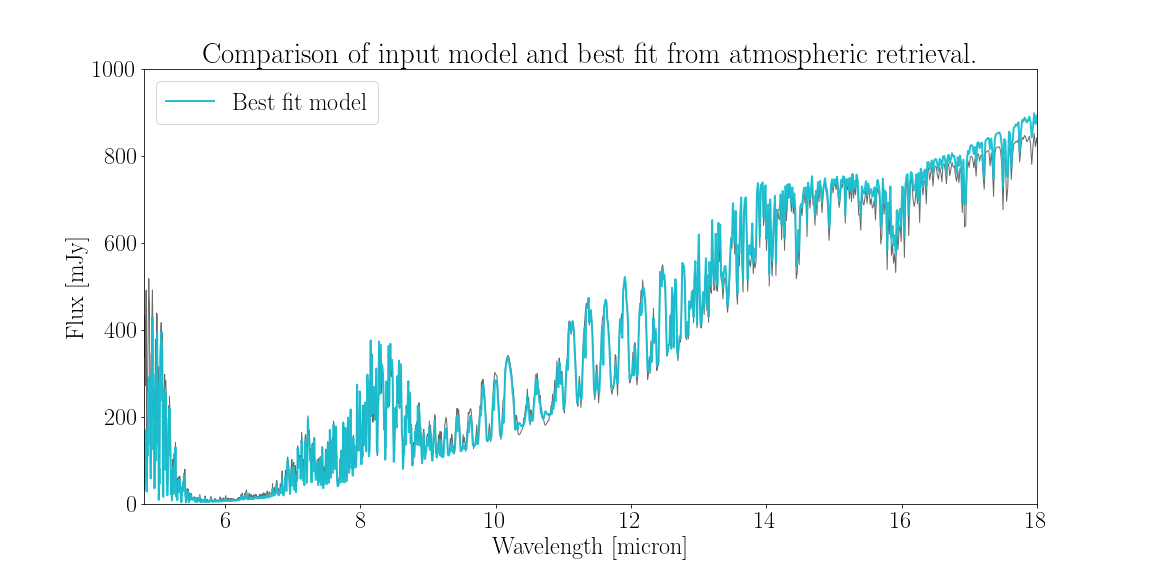
\includegraphics[width=\linewidth]{BestfitBrownDwarf_fringe}
	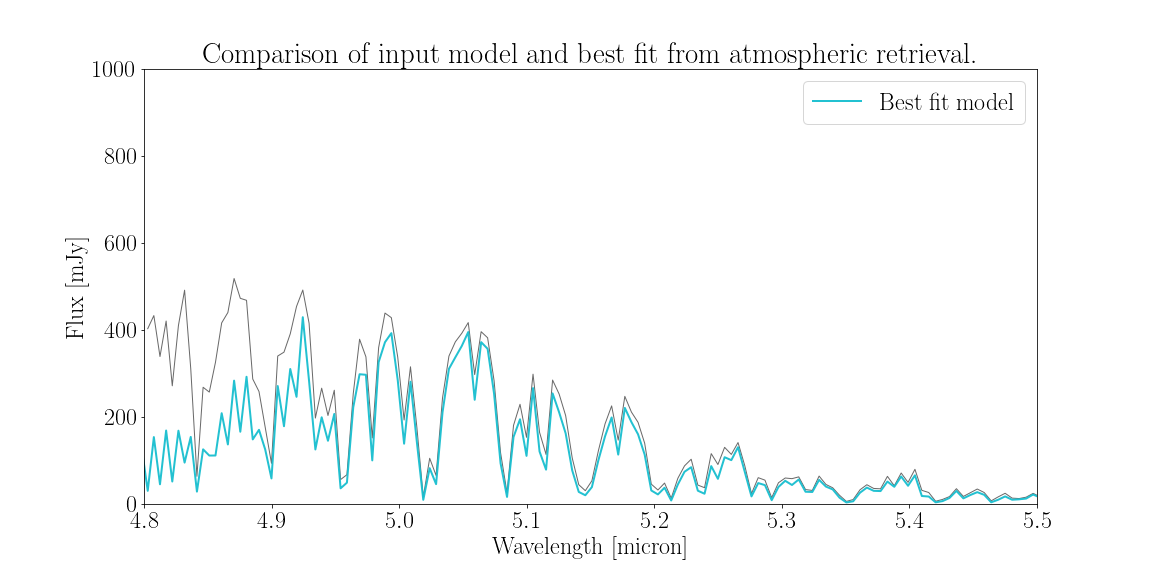
\includegraphics[width=\linewidth]{BestfitWISE0855}
	\caption{Best fit model for WISE0855}
	\label{fig:bestfitWISE}
\end{figure}
\subsection{Discussion}
% This all ignores inherent issues that may be present in petitRADTRANS. However, the purpose of this work is not to realistically model atmospheres, but rather to show the extent to which current tools can retrieve input parameters. Other works such as \parencite{Barstow2020} have compared various retrieval and modelling tools, finding that while generally similar results are obtained, there are scenarios where different tools lead to different posterior distributions. 